\documentclass[10pt,a4paper]{article}
\usepackage[utf8]{inputenc}
\usepackage[english]{babel}
\usepackage{amsmath}
\usepackage{amsfonts}
\usepackage{amssymb}
\usepackage{graphicx}
\usepackage[left=3.5cm,right=3.5cm,top=3cm,bottom=3cm]{geometry}

\usepackage{mathtools}

\usepackage{natbib}
\bibliographystyle{apalike}
%\bibliographystyle{unsrtnat}

\author{Fabian Schubert}
\title{Driven Random Dynamic Reservoir with Homeostatic Variance Control}

%\def\avgt#1{\langle {#1} \rangle_T}
%\def\avgp#1{\langle {#1} \rangle_P}

\newcommand{\avgt}[1]{\left< #1 \right>_T}
\newcommand{\avgp}[1]{\left< #1 \right>_P}

\parskip=5pt

\begin{document}
\begin{center}
\begin{LARGE}
\textbf{Driven Random Dynamic Reservoir with Homeostatic Variance Control}\\
\end{LARGE}
\end{center}

\section{Model Description}

\subsection{Dynamics}
\begin{align}
y_i^{t+1} &= \mathrm{tanh}\left( a_i^t I_i^{t+1} \right) \label{eq:reserv_dynamics}\\
I_i^{t+1} &= \sum_{j=1}^{N} W_{ij} y_j^t + E_i^{t+1} \label{eq:input_dynamics} \\
b_i^{t+1} &= b_i^t + \epsilon_{b} \left[ \avgt{y_i} - \mu_{t} \right] \\
a_i^{t+1} &= a_i^{t} + \epsilon_{a} \left[ \sigma_{t}^2 - \left( y_i^t - \overline{y}(t)_i\right)^2 \right] \label{eq:gain_dynamcis} \\
\overline{y}^{t+1}_i &= \epsilon_{\rm trail} \left[ y_i^{t+1} - \overline{y}^{t}_i\right]
\end{align}

We denote by $\avgt{\cdot}$ an average over time and by $\avgp{\cdot}$ over the population.

\subsection{Parameters / Settings}

$W_{ij}$ is a sparse random matrix with connection probability $p$. Nonzero entries were drawn from a Gaussian distribution $\mathcal{N}(\mu = 0,\sigma = \sigma_{W}/\sqrt{N p})$. Diagonal entries were always set to zero.


$E^t_{i}$ are random vectors of size $N$ with independent entries drawn from a Gaussian distribution $\mathcal{N}(\mu = 0,\sigma = \sigma_{\rm ext})$. External input is turned off after $t_0$.

By changing individual gain and bias values $a_i$ and $b_i$, the homeostatic control tries to drive the activity standard deviation and mean of every cell to the value given by $\sigma_{t}$ and $\mu_{t}$. However, these mechanisms are also switched off after $t_0$. This is done because we can assume that homeostatic processes would biologically act on much slower timescales than changes in input. Before $t_0$, we can set $\epsilon_{a}$ and $\epsilon_{b}$ to relatively high values to let homeostasis converge under external drive.

All parameters that were unchanged throughout all simulations are shown in Table \ref{tab:params}.

\begin{table}[h]
	\caption{Model Parameters}
	\centering
	\vspace{5pt}
	\begin{tabular}{ l | l | l | l | l | l | l | l }
		 $N$ & $p$ & $\sigma_{W}$ & $\epsilon_{b}$ & $\epsilon_{a}$ & $\epsilon_{\rm trail}$ & $\mu_{t}$ & $t_0$  \\
		\hline
		\hline
		\rule{0pt}{12pt}
		1000 & 0.1 & $ w_0 $ & $2\cdot 10^{-4}$ & $10^{-3}$ & $10^{-4}$ & 0 & $10^5$
	\end{tabular}
	\label{tab:params}
\end{table}

\section{Derivation of Gain Dynamics from Objective Function}
We would like to justify our choice of \eqref{eq:gain_dynamcis} by deriving an update rule from a suitable objective function $F_{\sigma}$:
\begin{equation}
F_{\sigma} = \left[\avgt{\left(y-\avgt{y}\right)^2} - \sigma^2_{t}\right]^2
\end{equation}
Using $\Delta a \propto - \frac{\partial F_\sigma}{\partial a}$:
\begin{align}
\Delta a &\propto a^{-1} \left[\sigma^2_{t} - \avgt{\left(y-\avgt{y}\right)^2}\right]\avgt{\left(y-\avgt{y}\right)\mathrm{arctanh}(y)\left(1-y^2\right)} \label{eq:gain_dynamics_obj_func1} \\
&=a^{-1} \left[\sigma^2_{t} - \avgt{\left(y-\avgt{y}\right)^2}\right]\mathrm{Cov}\left[ y,\mathrm{arctanh}(y)\left(1-y^2\right) \right]_T \label{eq:gain_dynamics_obj_func2}
\end{align}
The sign in the covariance term in \eqref{eq:gain_dynamics_obj_func2} determines whether the dynamics given in \eqref{eq:gain_dynamcis} are recovered, or if the gain adaptation is reversed. Intuitively, it indicates if increasing $a$ broadens or narrows the output distribution. Fig.~\ref{fig:gain_cov} illustrates that a positive covariance is always ensured if the activity remains within the region highlighted in gray, which is approximately given by $(-0.648,0.648)$. For symmetry reasons, $\mathrm{Cov}\left[ y,\mathrm{arctanh}(y)\left(1-y^2\right) \right]_T \geq 0$ also holds for distributions exceeding this bound if they are symmetric around $y=0$. In our numerical simulations, this symmetry condition was fulfilled due to the Gaussian distribution of the neural input, which was centered around zero. This allowed us to reduce dynamics to the essential term $\left[\sigma^2_{t} - \avgt{\left(y-\avgt{y}\right)^2}\right]$.

\begin{figure}
	\centering
	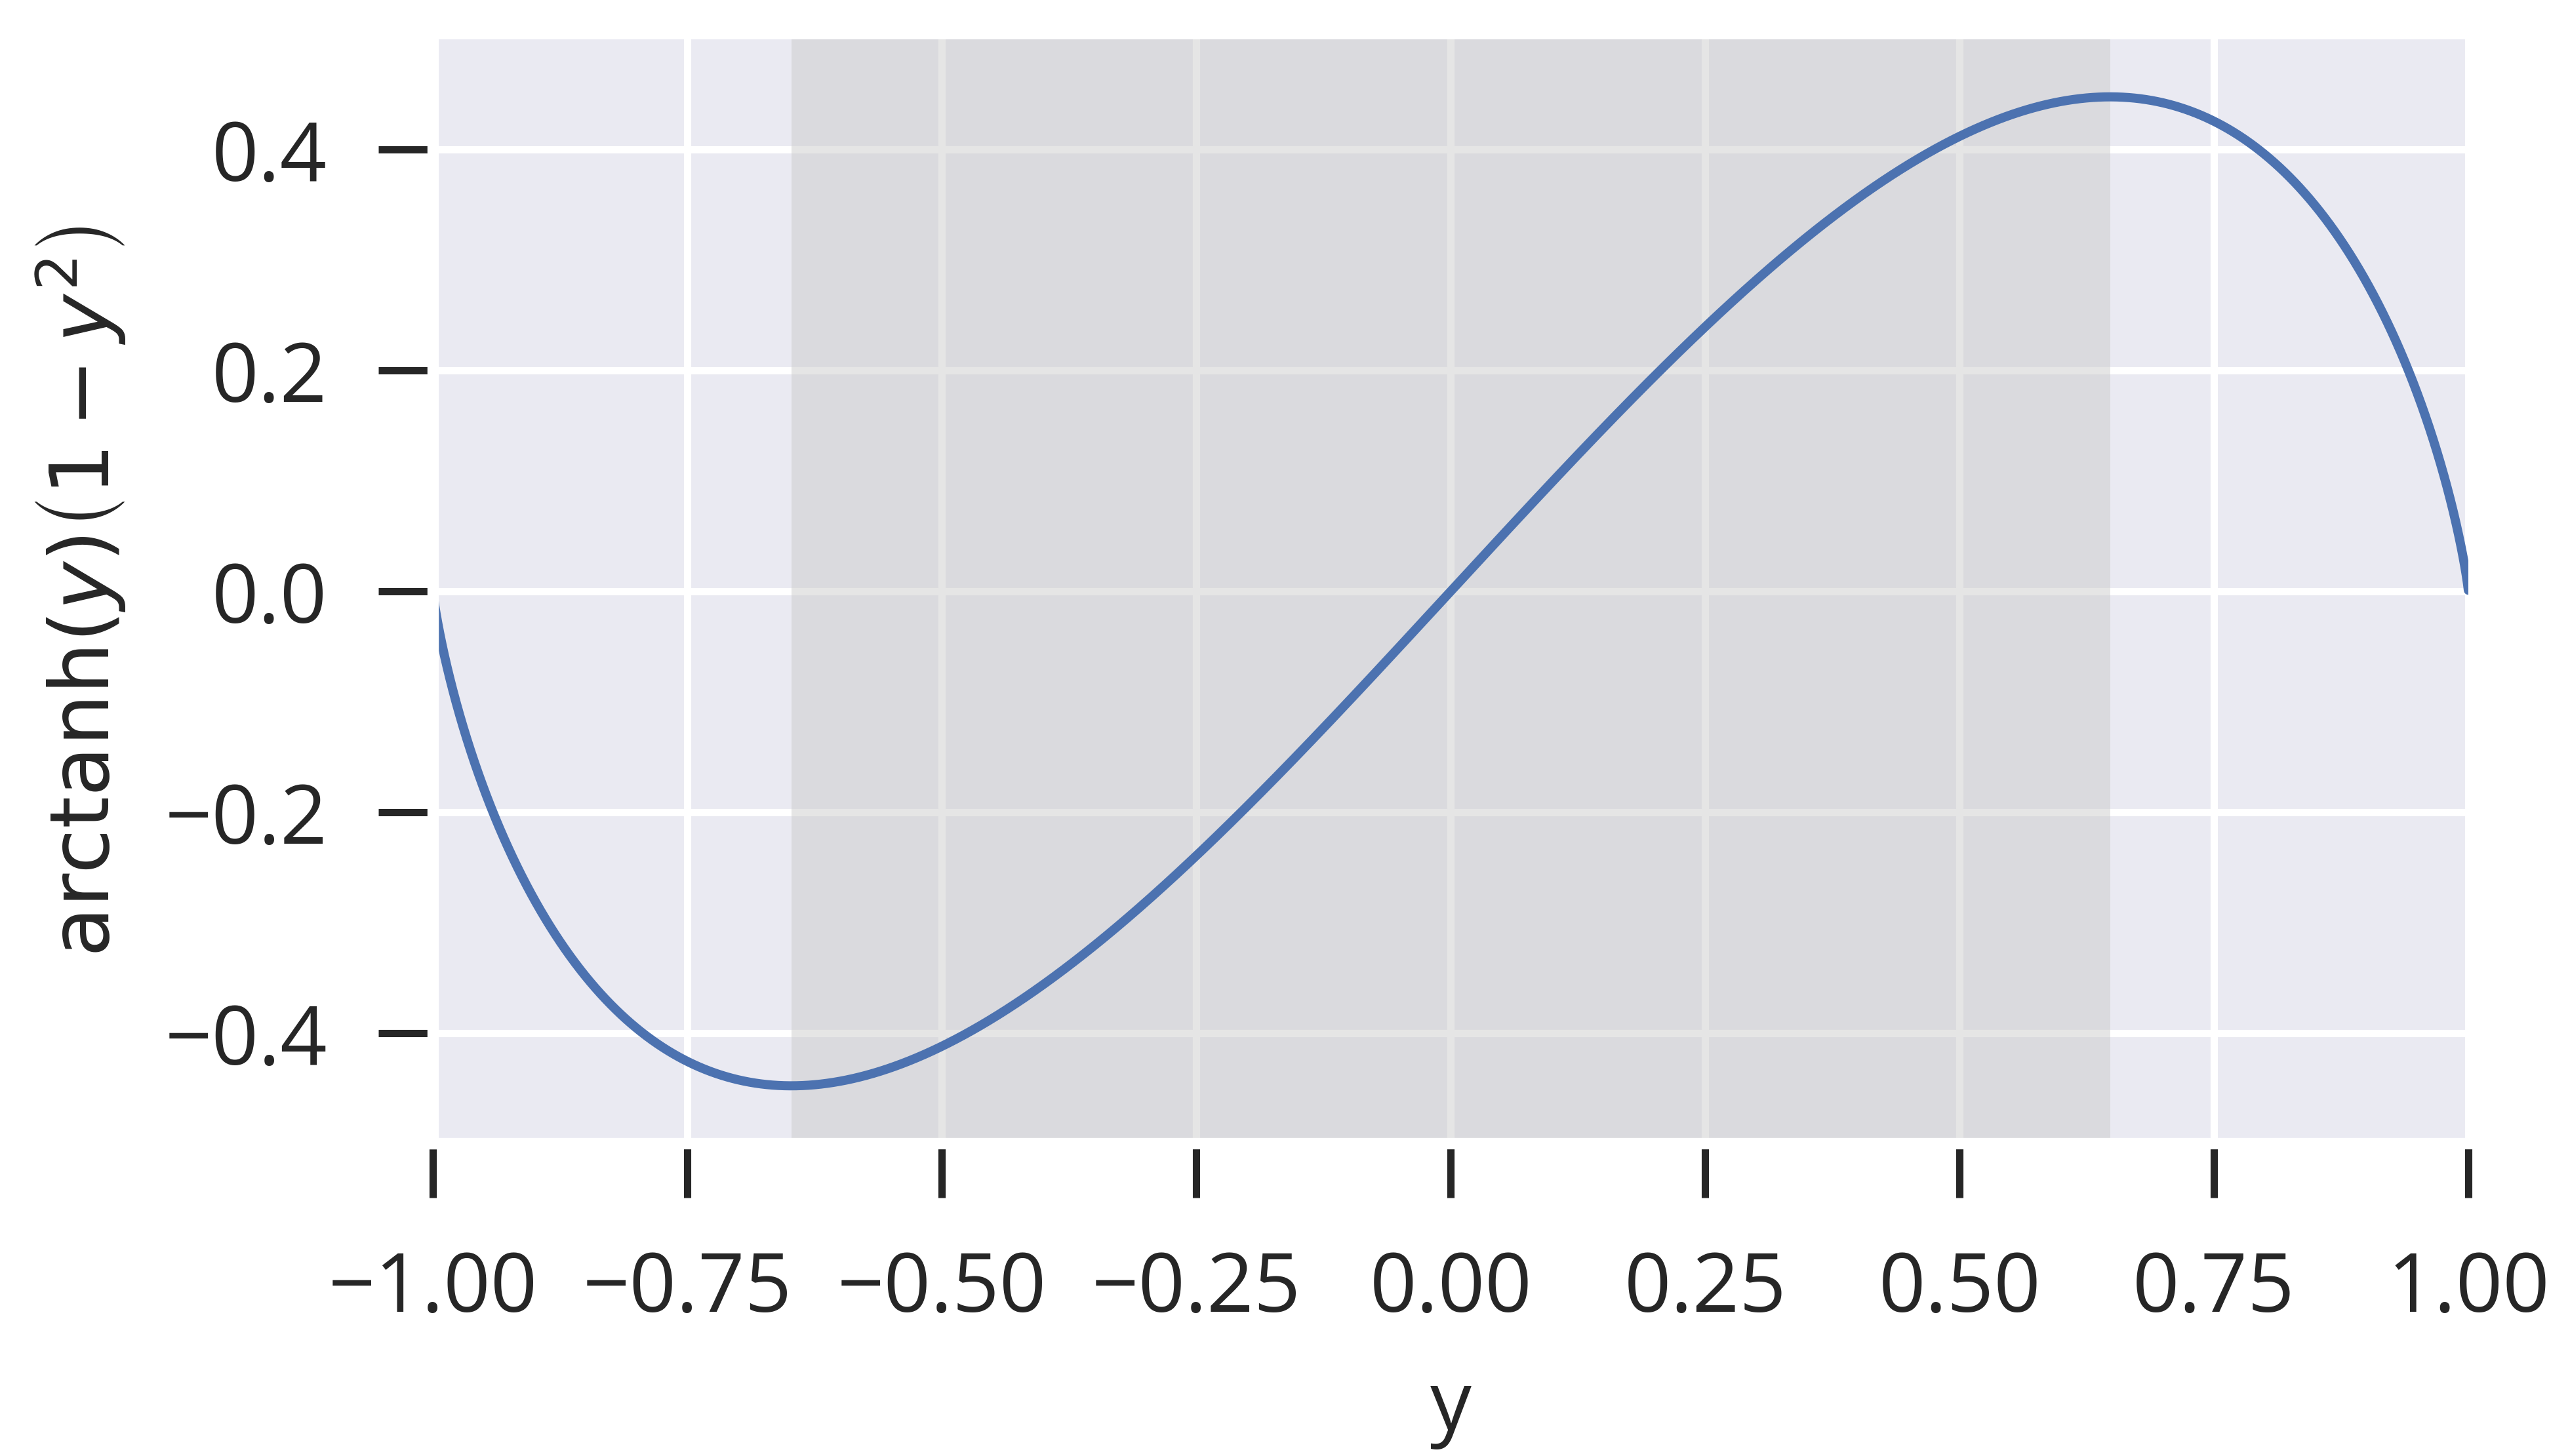
\includegraphics{../plots/gain_grad_descent.png}
	\caption{Covariance term of \eqref{eq:gain_dynamics_obj_func2}. If $y$ is bound within the gray area, positive covariance is ensured.}
	\label{fig:gain_cov}
\end{figure}

\section{Results}
Exemplary results are shown in Fig. \ref{fig:ex_results}.

\begin{figure}[h]
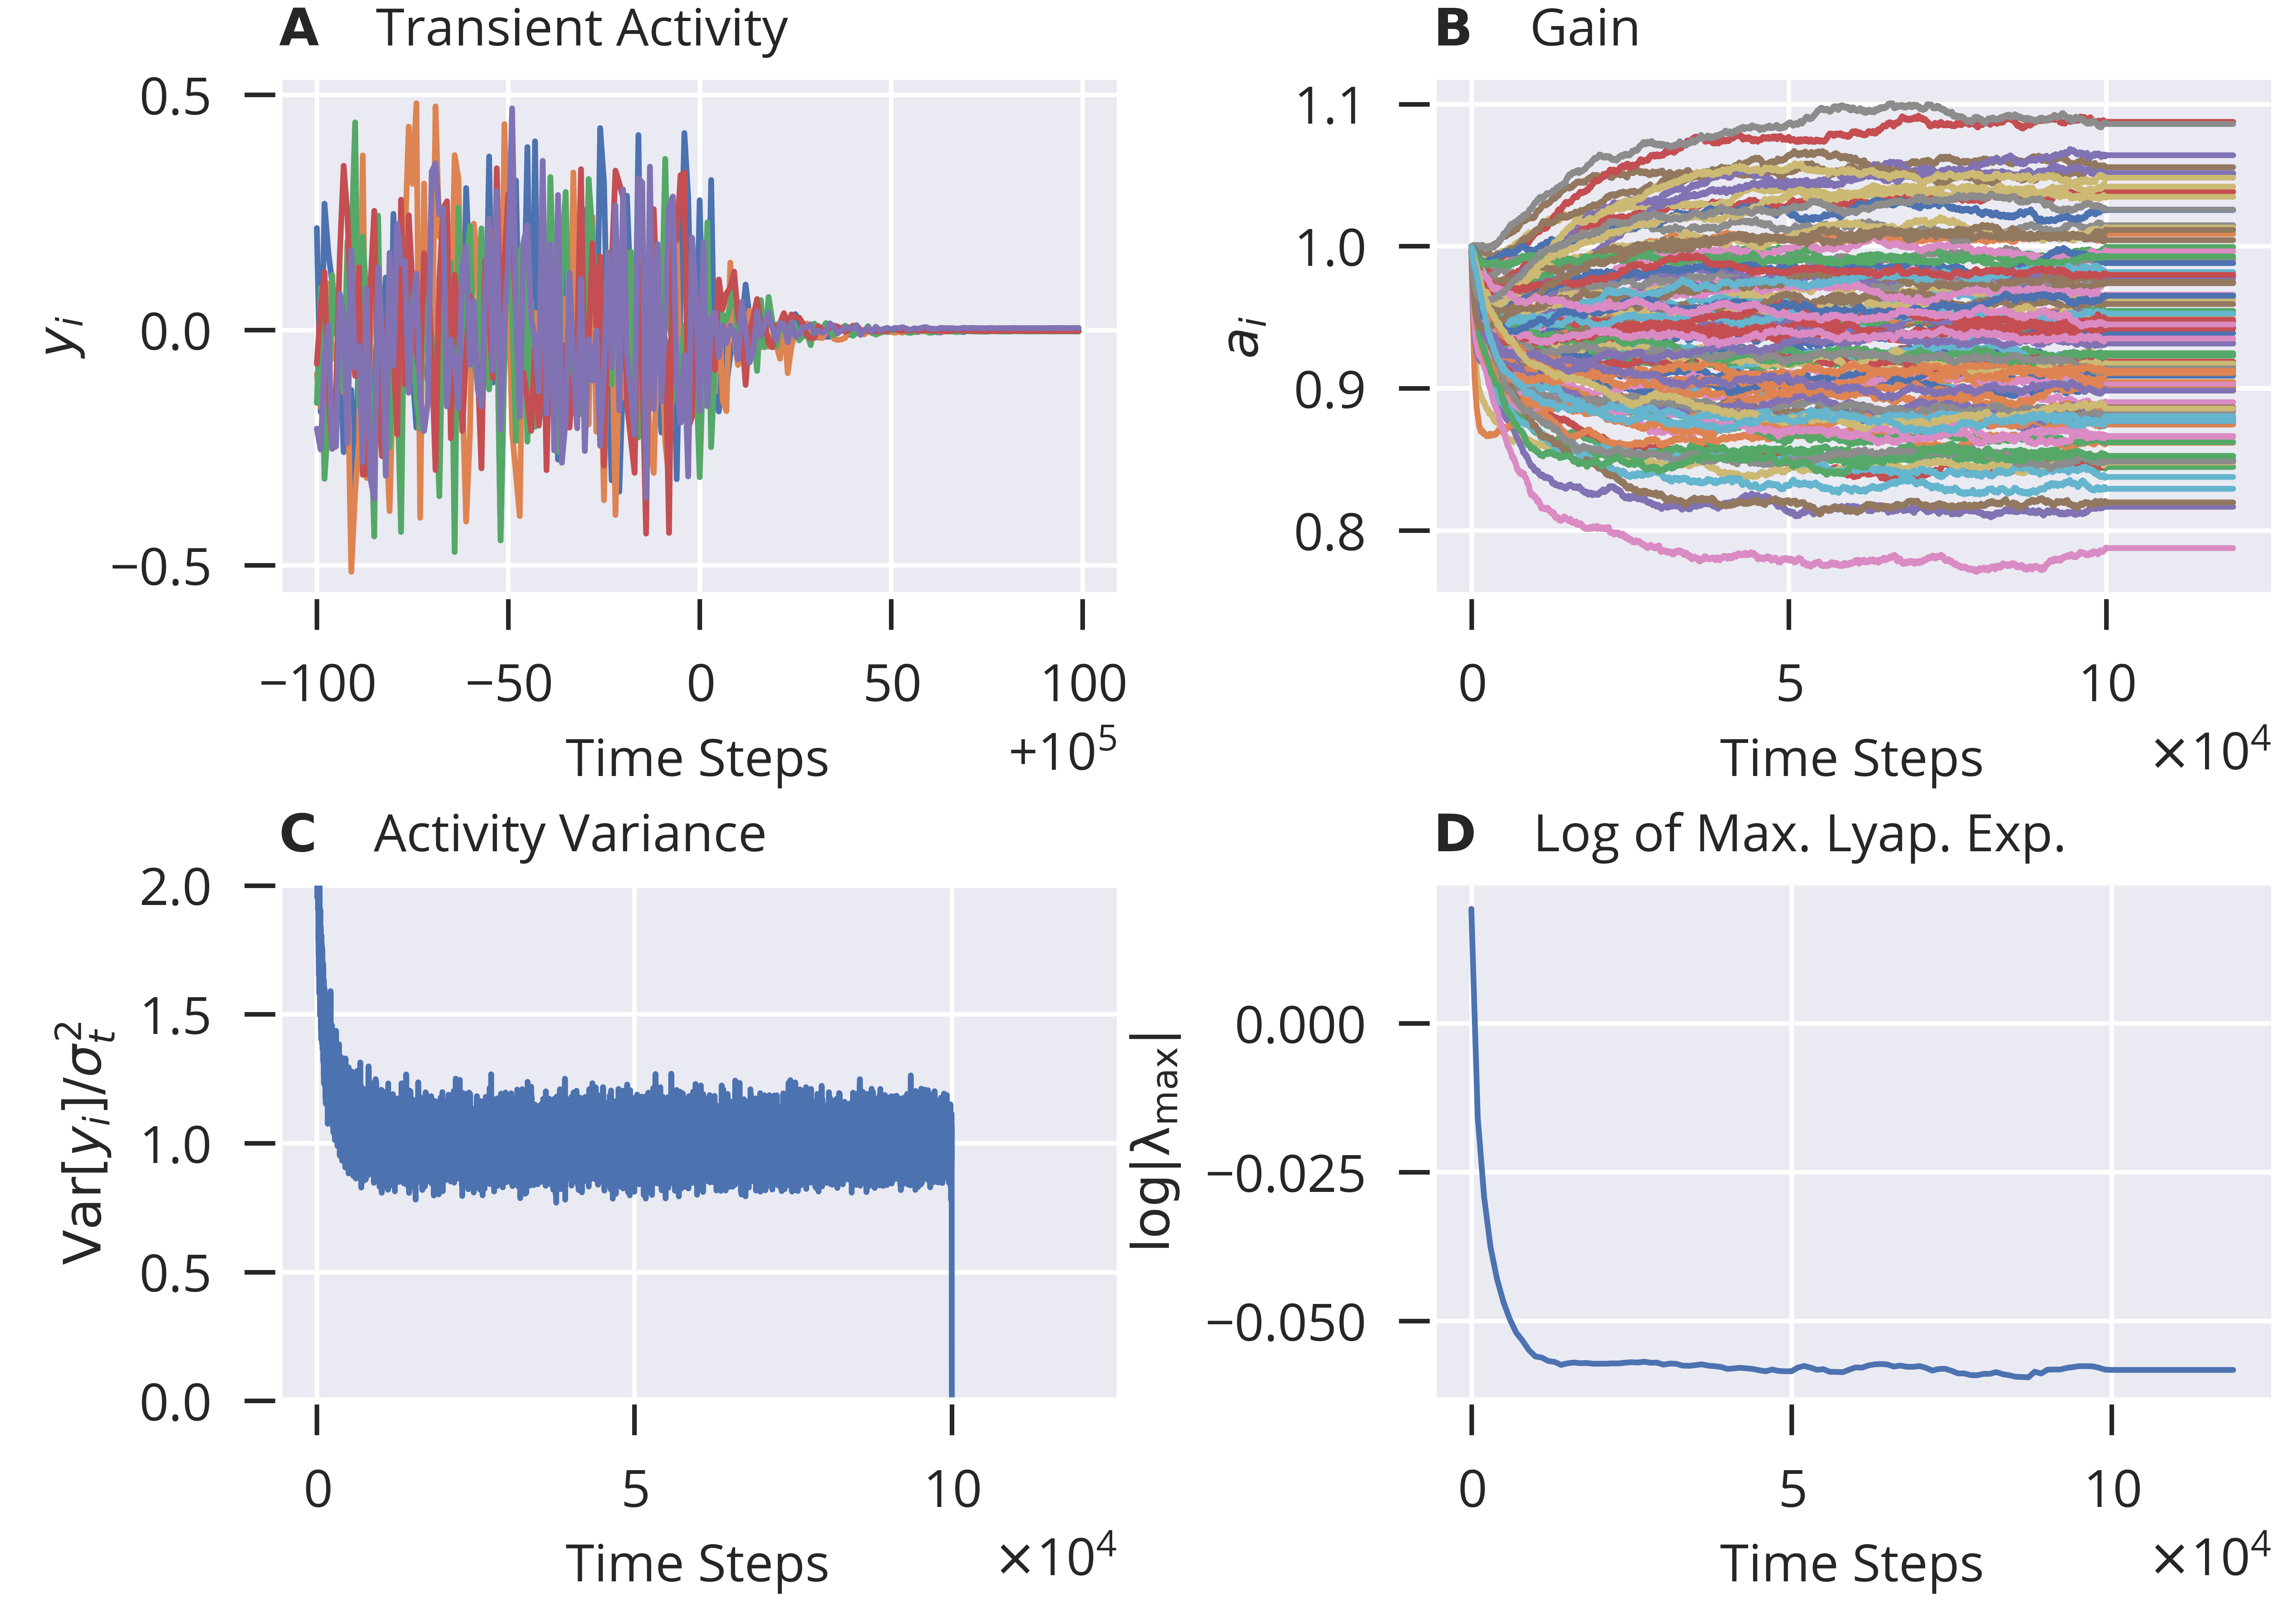
\includegraphics[width=\textwidth]{../plots/res_comp.png}
\caption{{\bf A}: Sample of activity within $\left[ t_0 - 100, t_0 + 100 \right]$. {\bf B}: Gain dynamics of $N/10$ exemplary neurons. {\bf C}: Population mean of squared activity, normalized by target variance. {\bf D}: Log. of largest absolute value of eigenvalues of $a_i^t W_{ij} $. Standard parameters are as given in Table~\ref{tab:params}. Furthermore, $\sigma_{\rm ext} = 0.1$, $\sigma_{t} = 0.2$, total runtime $n_t = 1.2\cdot10^5$. }
\label{fig:ex_results}
\end{figure}

\begin{figure}[h]
	\centering
	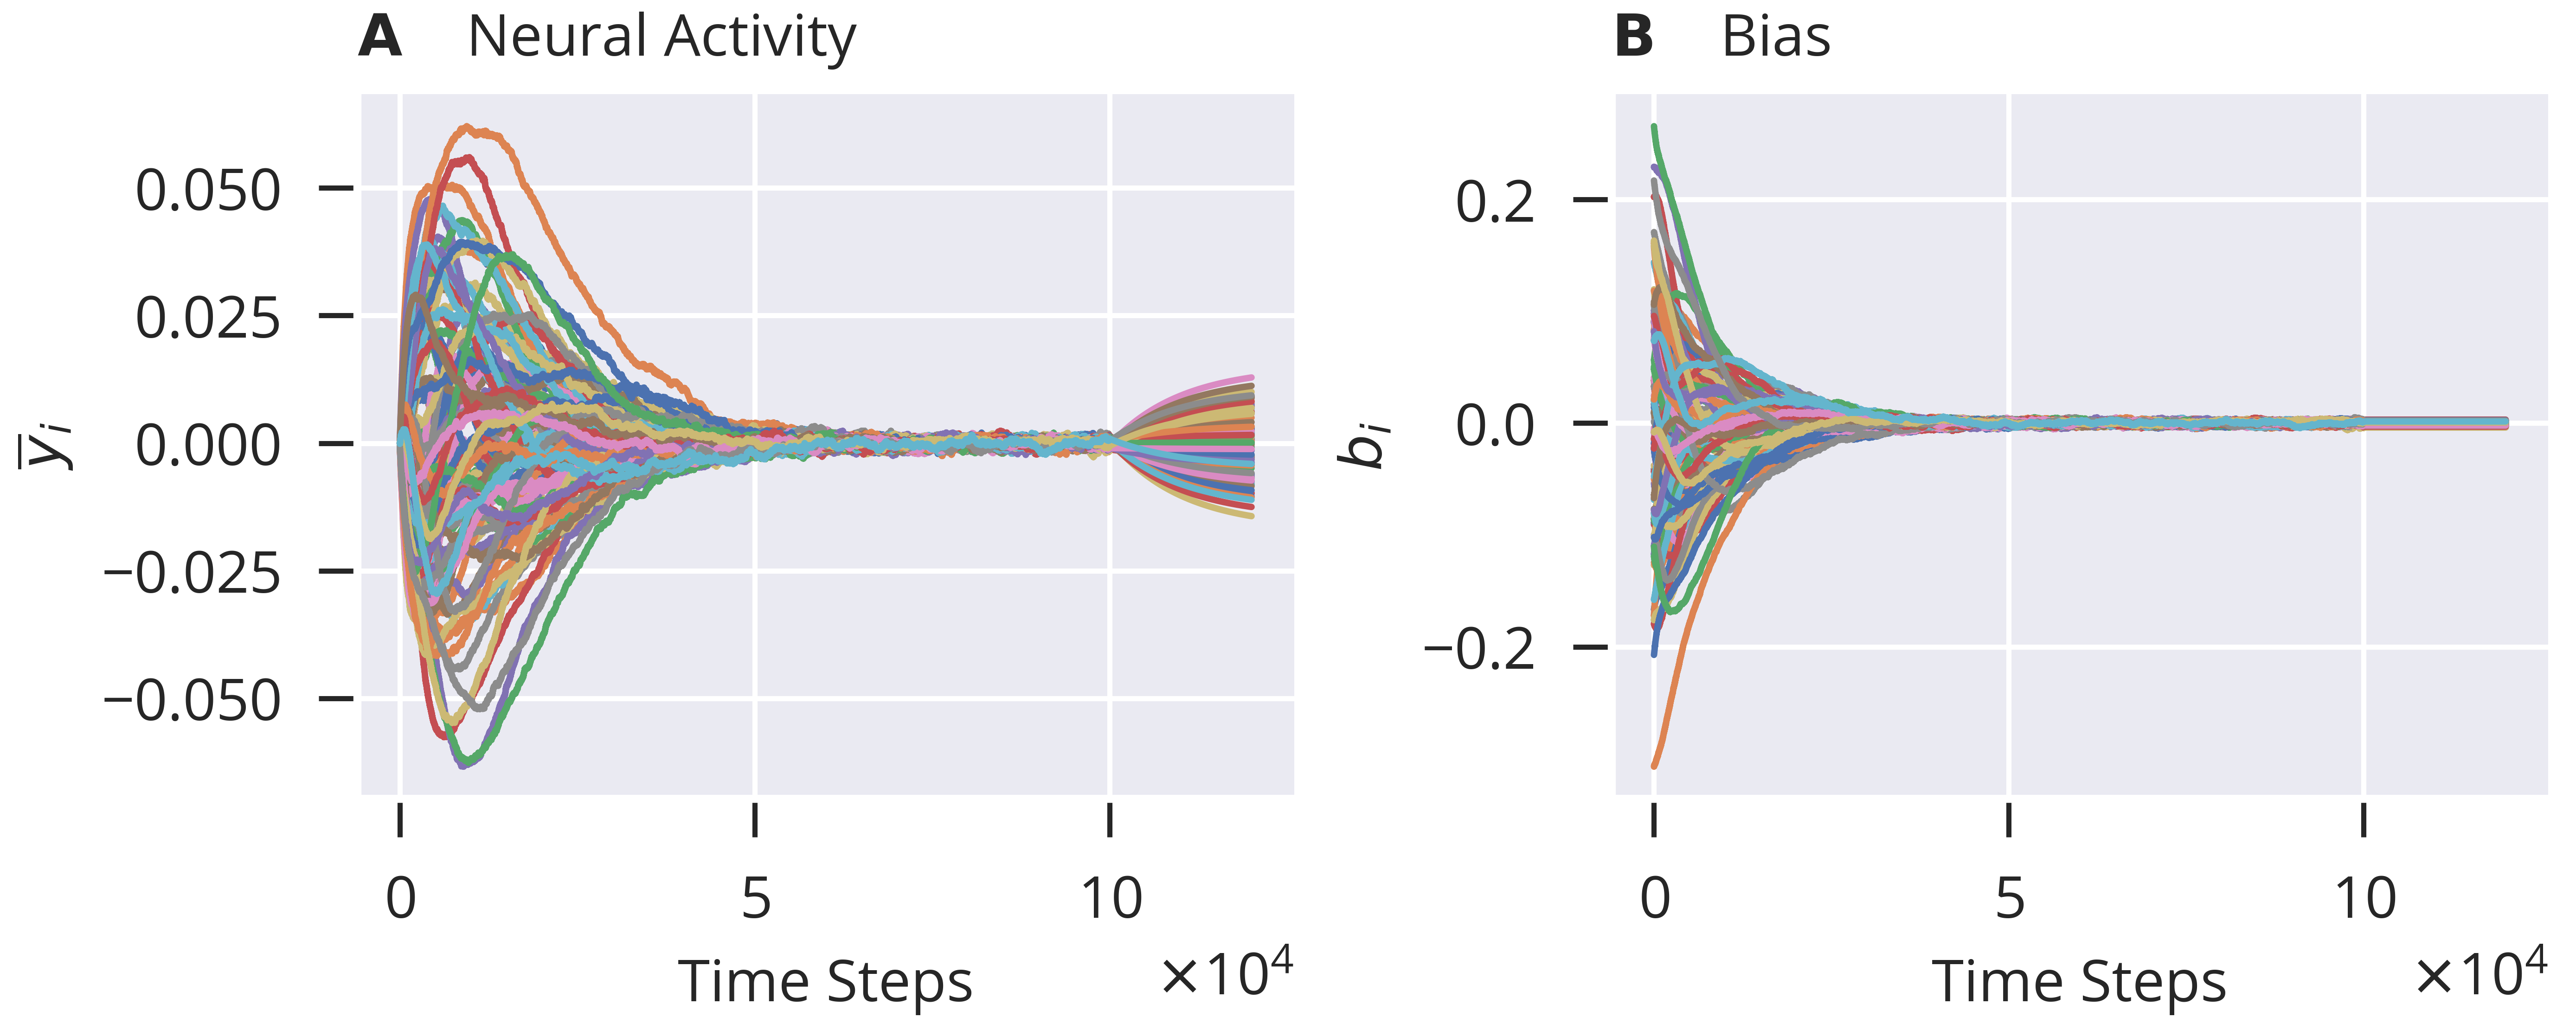
\includegraphics[width=\textwidth]{../plots/res_comp_act_bias.png}
	\caption{{\bf A}: Dynamics of population mean of neural activity. {\bf B}: Bias dynamics of $N/10$ exemplary neurons. }
\end{figure}

\section{Mean Field Approximation}

\begin{figure}[t]
	\centering
	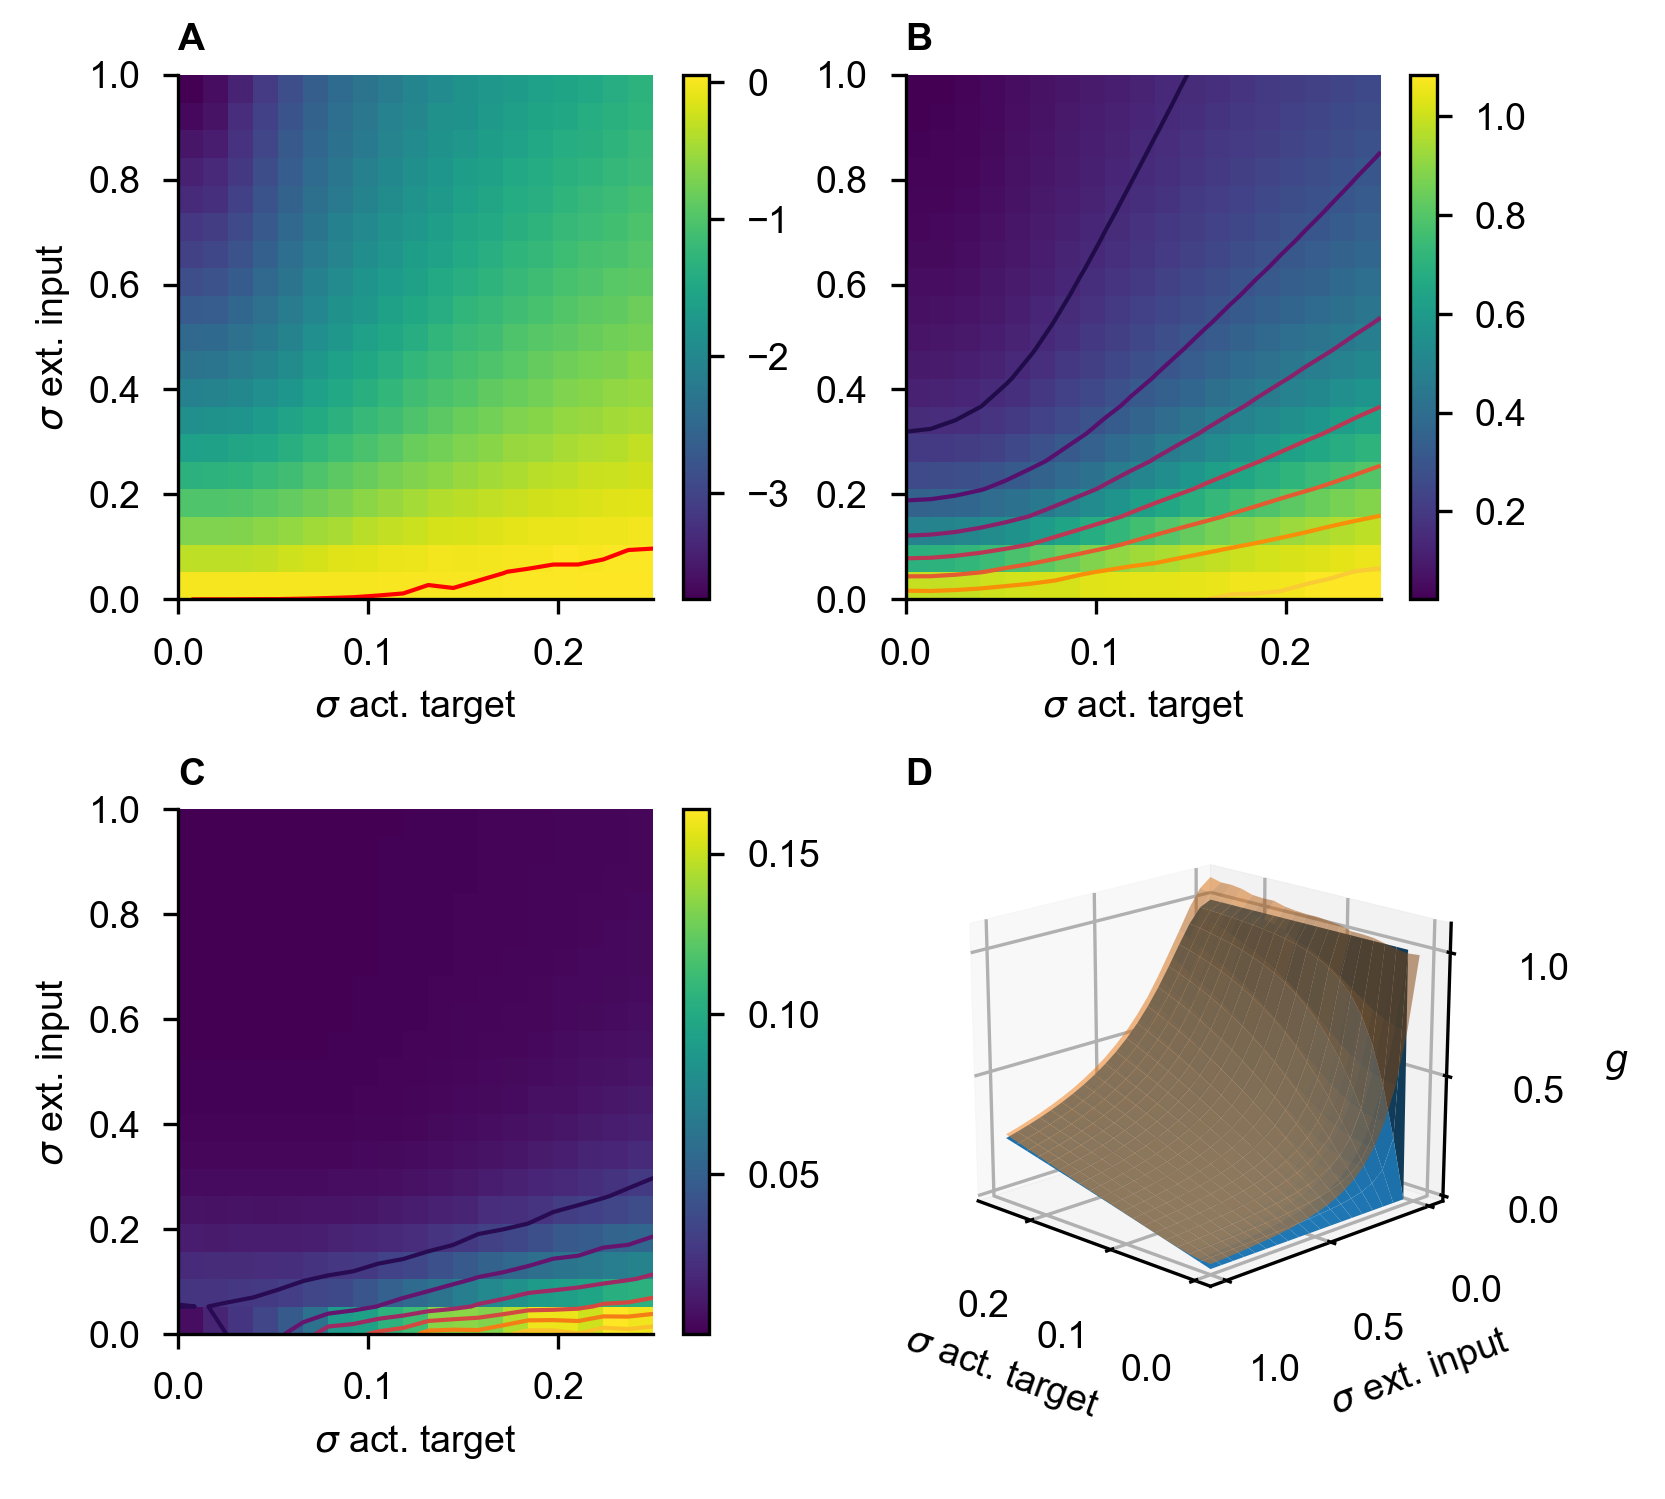
\includegraphics[width=\textwidth]{../plots/std_in_std_target_sweep_fig.png}
	\caption{Parameter sweep, run on a network with $N=1000$ (except {\bf C}). {\bf A}:~Log of largest absolute value of eigenvalues of $a_i W_{ij}$. Turquois dashed line marks the zero transition. {\bf B}:~$\avgp{a_i}$.  White dashed line marks the $\avgp{a_i} = 1$ transition. Turquois line as in {\bf A}. {\bf C}:~$\avgp{(a_i - \avgp{a_i})^2}$ as a function of $N$. {\bf D}:~Memory Capacity (color coded), zero transition of largest absolute eigenvalue (turquois line), maximal memory capacity for a given standard deviation of external drive (orange). Red line marks the loss of the echo state property.}
	\label{fig:gain_std_in_std_targ_sweep}
\end{figure}

\begin{figure}[t]
	\centering
	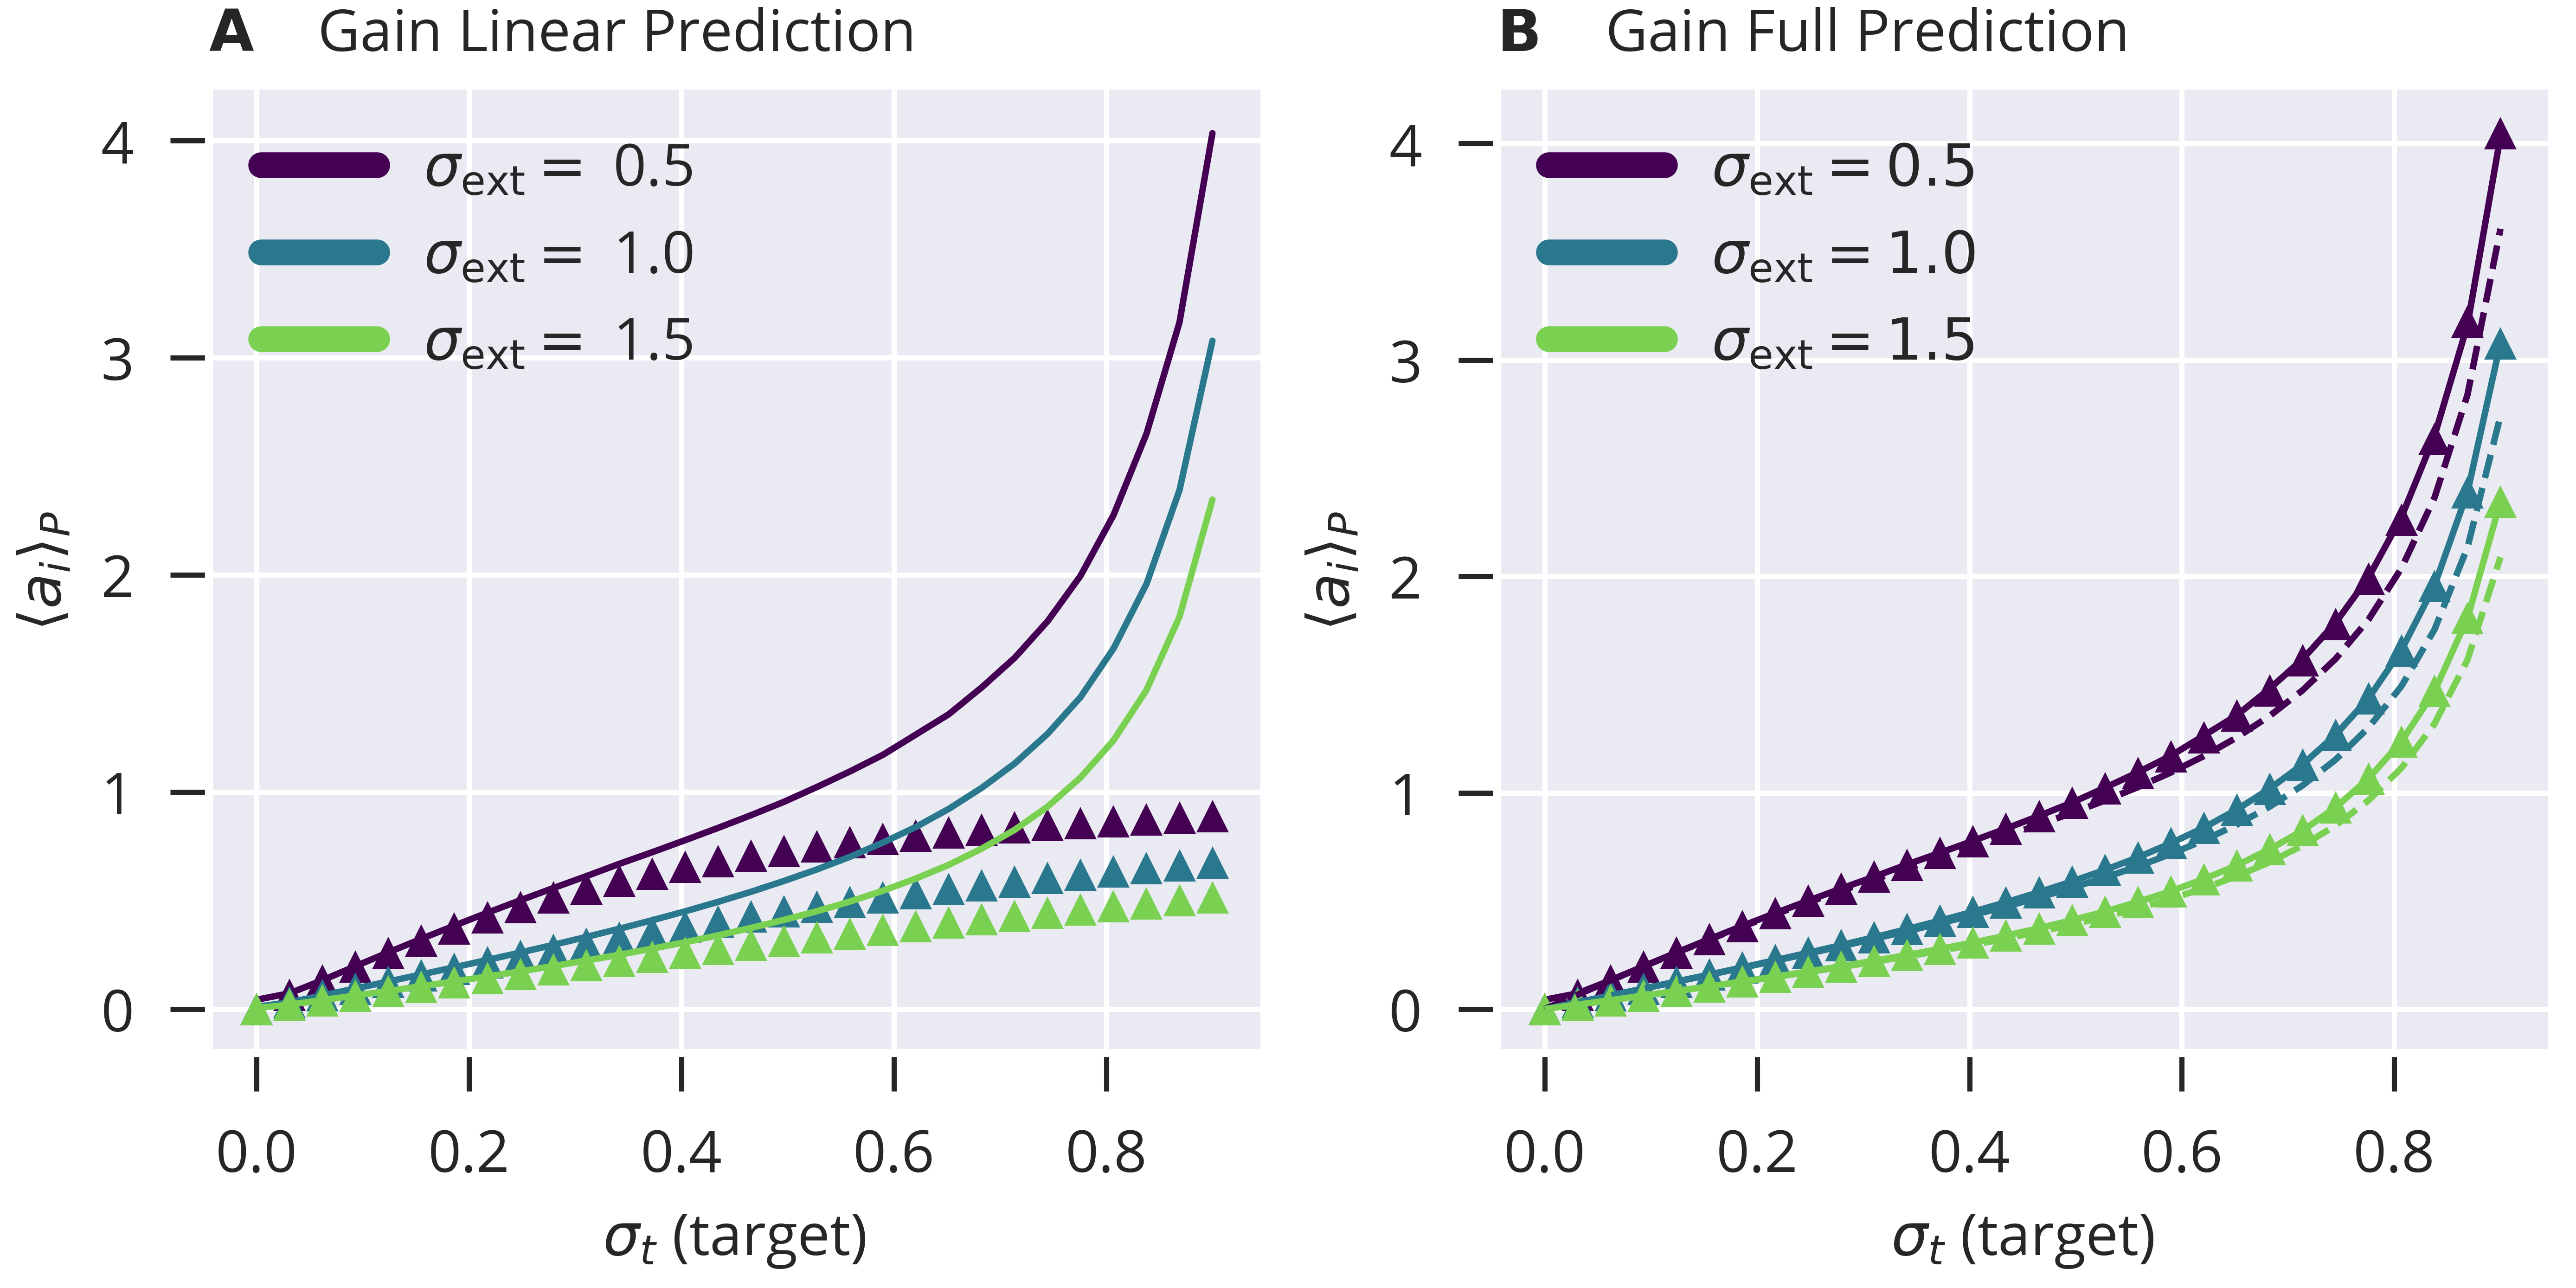
\includegraphics[width=\textwidth]{../plots/std_in_std_target_sweep_fig_cut.png}
	\caption{{\bf A}: Prediction of \eqref{eq:gain_pred} (triangles) and numerical result (lines) of $\avgp{a_i}$. {\bf B}: $\avgp{a_i}$ from the simulation matches the numerically determined solution of \eqref{eq:self-consistency_var_full}.}
\end{figure}

We would like to find an approximate relation between the gain resulting from homeostasis and the input and target variance. If we linearize the neural activation function and take an average over time, we get
\begin{align}
	\avgt{y_i^2} &= a_i^2 \avgt{\left(\sum_{j=1}^{N} W_{ij} y_j + E_i\right)^2} \label{eq:time_avg_act_var}\\
	&= a_i^2 \avgt{\left( \sum_{j=1}^{N} W_{ij} y_j \right)^2} + a_i^2 E_i^2 \\
	&= a_i^2 \sum_{j,k=1}^{N} W_{ij}W_{ik} \avgt{y_j x_k} + a_i^2 E_i^2 \; .
\end{align}
If we assume that the system is in a chaotic state we can set $\avgt{y_j x_k}=0$ for $j\neq k$. This leads to
\begin{equation}
	\avgt{y_i^2} = a_i^2 \left( \sum_{j=1}^{N} W_{ij}^2 \avgt{y_j^2} + \sigma_{\rm ext}^2 \right)
\end{equation}
where we have assumed $\avgt{E_i} = 0$ for all $i$.

By design, our homeostatic mechanism fixes all $\avgt{y_i^2}$ to $\sigma_{t}^2$. Thus,
\begin{align}
	\sigma_{t}^2 &= a_i^2 \left( \sigma_{t}^2 \sum_{j=1}^{N} W_{ij}^2 + \sigma_{\rm ext}^2 \right) \\ 
	a_i &= \left(\sum_{j=1}^{N} W_{ij}^2 + \sigma_{\rm ext}^2 / \sigma_{t}^2\right)^{-1/2} \; .
\end{align}

Since $W_{ij}$ is a random Gaussian matrix with variance $\sigma_W^2 = w_0^2/\left( N p \right)$ , $\sum_{j=1}^{N} W_{ij}^2$ follows a $\chi^2$ - distribution with variance $\frac{2N p \sigma_{W}^2}{N^2 p^2} = \frac{2 \sigma_{W}^2}{N p}$. For $N \rightarrow \infty $, its variance vanishes and consequently, all $a_i$ converge to the same value, namely 
\begin{equation}
	a = \left(\sigma_{W}^2 + \sigma_{\rm ext}^2 / \sigma_{t}^2\right)^{-1/2} \; . \label{eq:gain_pred}
\end{equation}
This equation predicts that $a$ should not change if the ratio between target and input variance remains constant. We ran a parameter sweep over $\sigma_{\rm ext}$ and $\sigma_{t}$ with a network of $N = 1000$ neurons and looked at the resulting distribution of gains and the maximal Lyapunov exponent. Importantly, this approximation suggests that the network should tune into a subcritical configuration for any non-vanishing external input. Even though this is not strictly verified in the numerical simulation, see Fig.~\ref{fig:gain_std_in_std_targ_sweep}A, it holds for the majority of $ \sigma_{\rm ext}$/$\sigma_{t}$ combinations.

\subsection{Self-Consistency Equation with Full Activation Function}
If we do not restrict ourself to a linearized version of the activation function, \eqref{eq:time_avg_act_var} becomes
\begin{equation}
	\avgt{y_i^2} = \avgt{\tanh\left(a_i\left(\sum_{j=1}^{N} W_{ij} y_j + E_i\right)\right)^2} \; .
\end{equation}
Again, assuming that $\avgt{y_j x_k}=0$ for $j\neq k$ and $N \rightarrow \infty$, the sum of weight and inputs follows a Gaussian distribution $\mathcal{N}\left(\mu = 0, \sigma = \sqrt{\sigma^2_{W}\sigma^2_{t} + \sigma^2_{\rm ext}}\right)$. Replacing the time average with an integral over the distribution of the input, we arrive at the full self-consistency equation
\begin{equation}
	\sigma^2_{t} = \int_{-\infty}^{\infty}  \tanh^2\left(ay\right) \mathcal{N}\left(y, \mu = 0, \sigma = \sqrt{\sigma^2_{W}\sigma^2_{t} + \sigma^2_{\rm ext}}\right)	\mathrm{d}y \label{eq:self-consistency_var_full}
\end{equation}

As a second order approximation with respect to $\tanh$, we can use $\tanh^2(y) \approx y^2 - \frac{2}{3} y^4$ in the integral, which gives

\begin{align}
\sigma_{t}^2 &\approx \frac{1}{a\sqrt{2 \pi}\sigma_{\rm total}}\int_{-\infty}^{\infty}\left( y^2 - \frac{2}{3}y^4\right)\exp\left( \frac{-y^2}{2a^2\sigma_{\rm total}^2}\right) \mathrm{d}y \\
&= a^2\sigma_{\rm total}^2 - 2a^4\sigma_{\rm total}^4 \\
&= a^2\left( \sigma^2_{W}\sigma^2_{t} + \sigma^2_{\rm ext} \right) - 2a^4 \left( \sigma^2_{W}\sigma^2_{t} + \sigma^2_{\rm ext} \right)^2 \label{eq:sec_order_approx_consistency}
\end{align}
where we have defined $\sigma_{\rm total} = \sqrt{\sigma^2_{W}\sigma^2_{t} + \sigma^2_{\rm ext}}$ for convenience. Note that neglecting the second term on the right hand side of \eqref{eq:sec_order_approx_consistency} reduces the equation to \eqref{eq:gain_pred}. Since this first order approximation does not explain the $a=1$ transition traced in Fig.~\ref{fig:gain_std_in_std_targ_sweep}B as a dashed blue line, we were particularly interested in the solution of \eqref{eq:sec_order_approx_consistency} for $a=1$. Moreover, we set $\sigma_{W}=1$ as in the simulations. We therefore had to solve
\begin{equation}
	\sigma_{t}^4 + \sigma_{\rm ext}^4 + 2\sigma_{t}^2\sigma_{\rm ext}^2 - \frac{\sigma_{\rm ext}^2}{2} = 0 \; .
\end{equation}
This equation can be rearranged to
\begin{equation}
	\left[\left(\sigma_{\rm ext} - \frac{1}{\sqrt{8}}\right)^2 + \sigma_{t}^2 - \frac{1}{8}\right]\left[\left(\sigma_{\rm ext} + \frac{1}{\sqrt{8}}\right)^2 + \sigma_{t}^2 - \frac{1}{8}\right] = 0 \; . \label{eq:circles_solution_form}
\end{equation}
From this form we can see that the solution set consists of two circles with radius $1/\sqrt{8}$ in the $\sigma_{t}$, $\sigma_{\rm ext}$ space, centered around $\sigma_{t} = 0$, $\sigma_{\rm ext} = \pm 1/\sqrt{8}$. Fig.~\ref{fig:crit_transition_2nd_order_approx} shows a comparison between this approximation and the simulation.

\begin{figure}
	\centering
	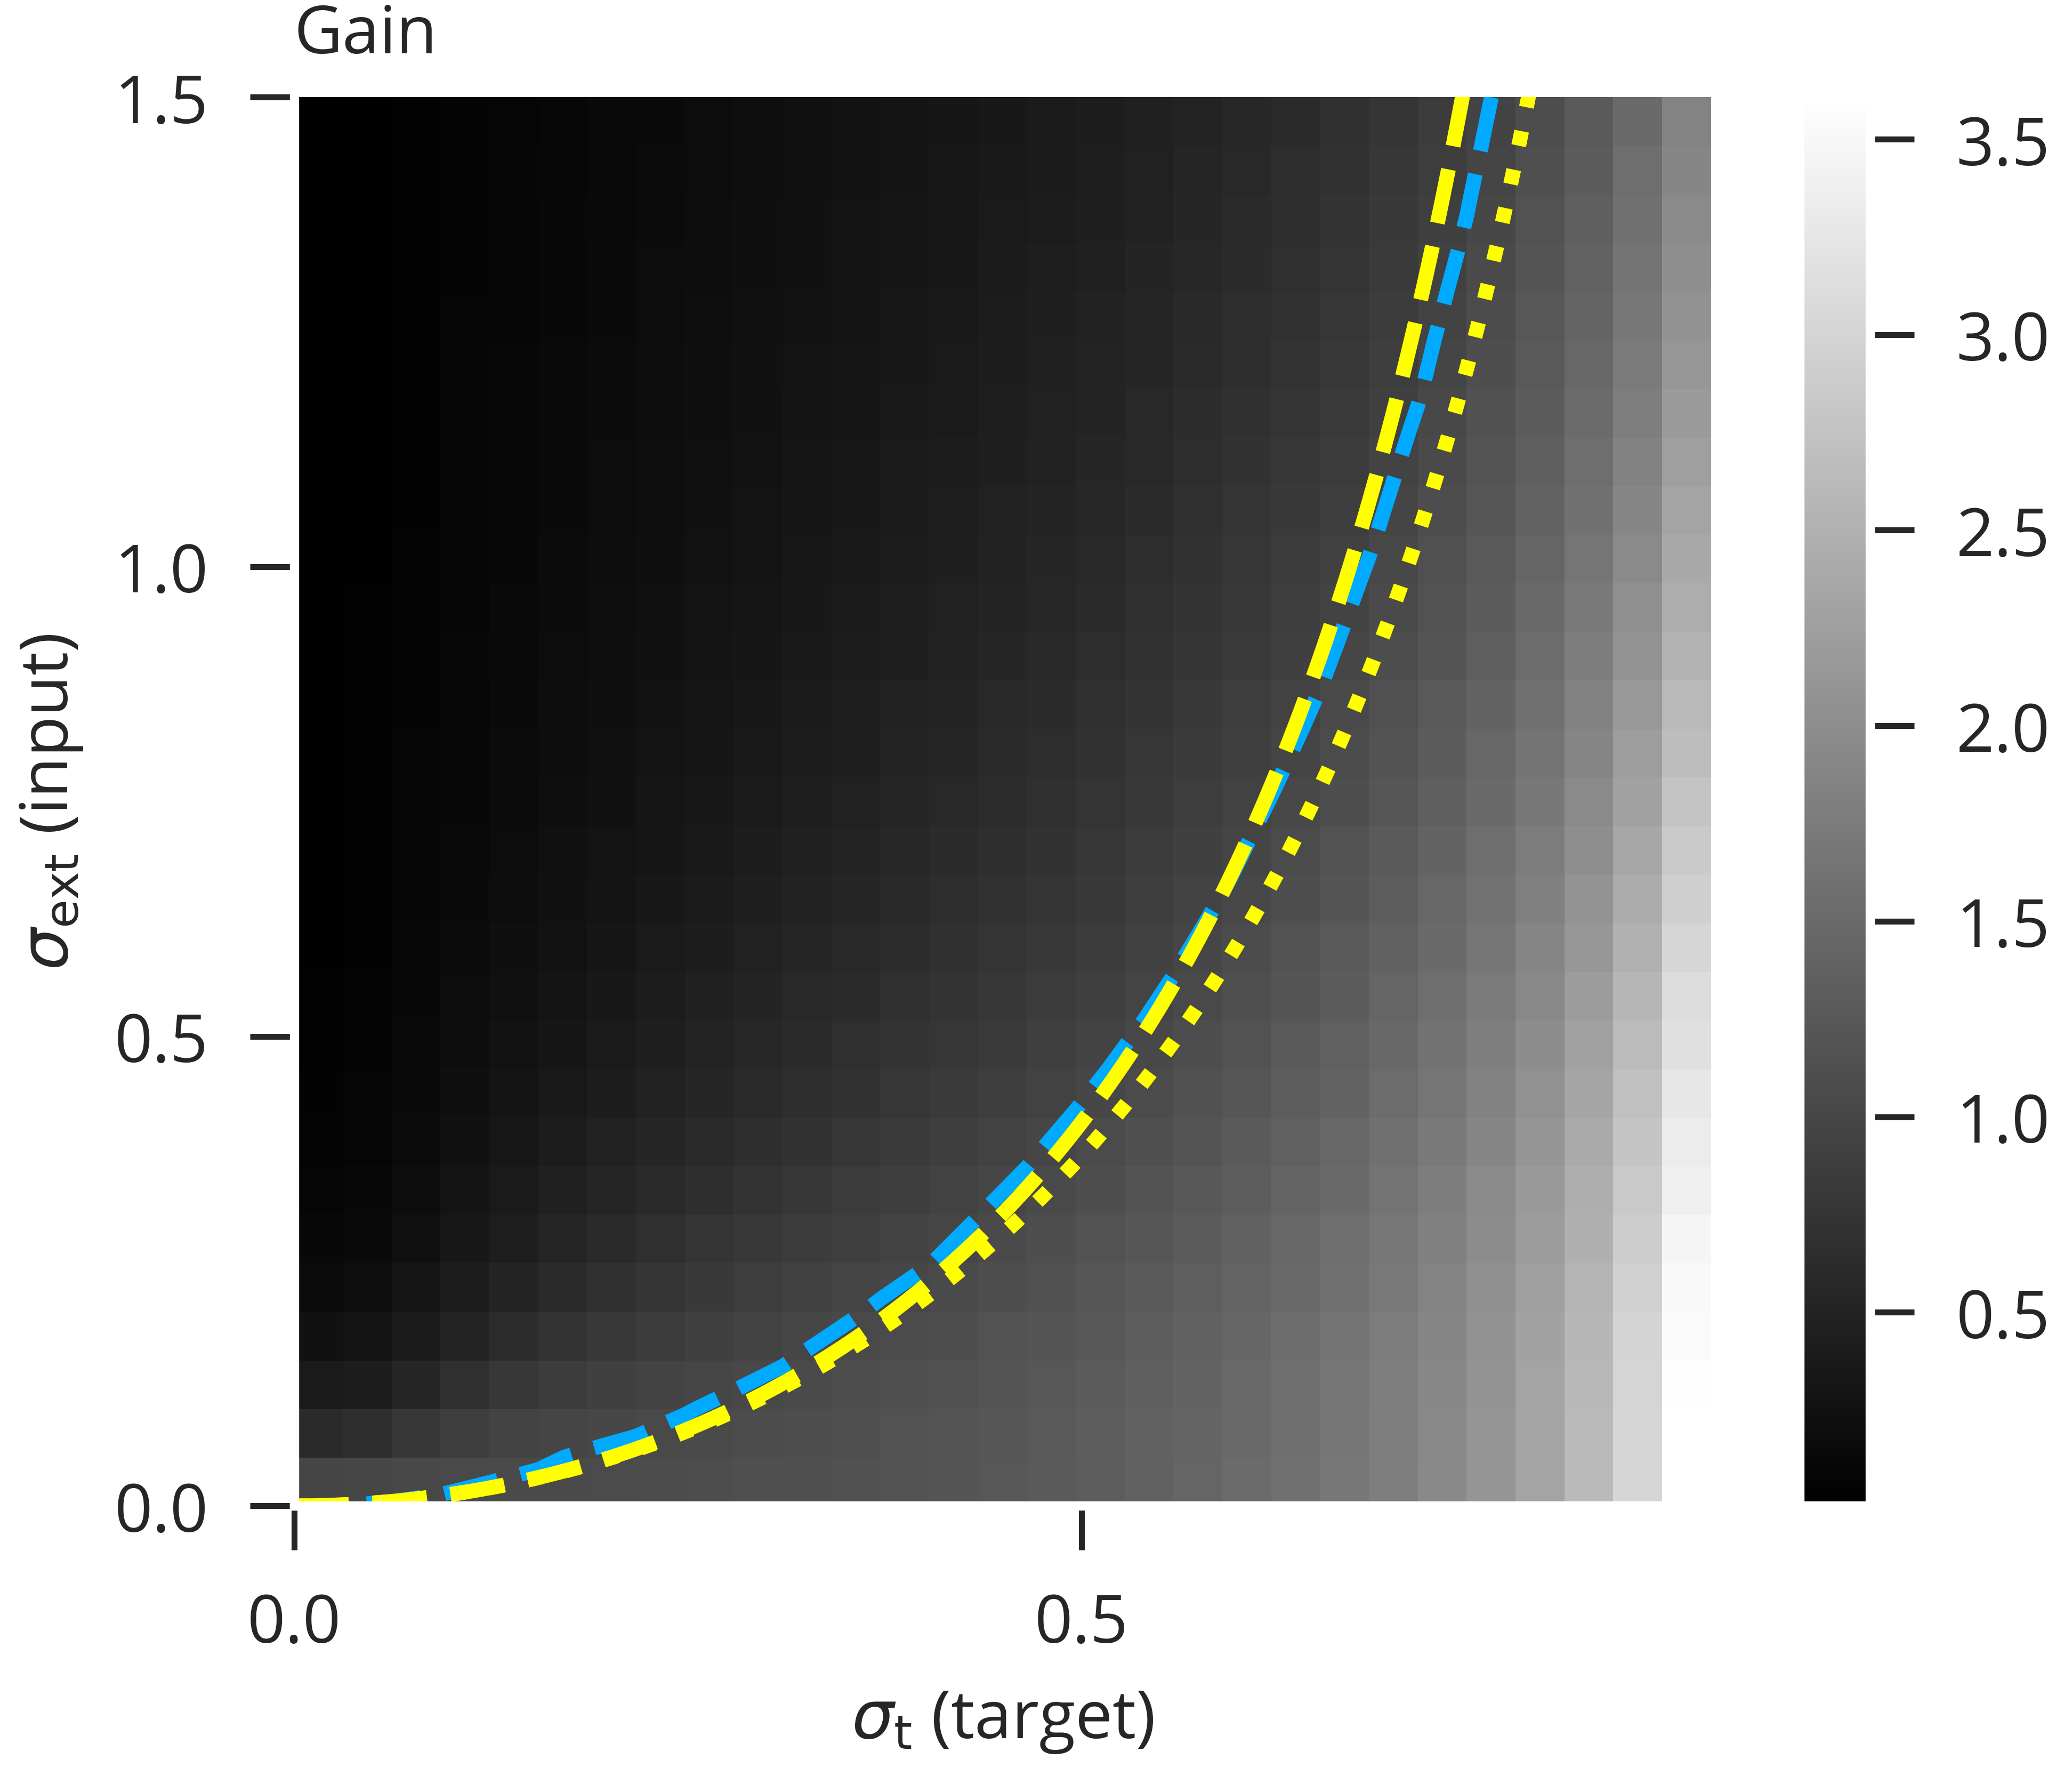
\includegraphics{../plots/crit_transition_2nd_order_approx.png}
	\caption{Comparison of the $\avgp{a_i} = 1$ transition (blue) shown in Fig.~\ref{fig:gain_std_in_std_targ_sweep}B and the second order approximate solution (yellow) given by \eqref{eq:circles_solution_form}. }
	\label{fig:crit_transition_2nd_order_approx}
\end{figure}

\section{Behavior for Input with Correlations Across Time/Population}

{\bf Test with e.g. Ornstein-Uhlenbeck Process and/or dominant princ. comp. in input space}

\section{Related Literature}

The effect of homoestatic mechanisms onto echo state network performance has been investigated in several works. A common approach derives dynamic adaptation rules from the minimization of a functional (usually KL-divergence) of an empirical estimate of each neuron's output distribution and a target PDF [\cite{Triesch_2007, Schrauwen_2008, Boedecker_2009}].

On the relation between Echo State Property and Input Signal Properties: \cite{Manjunath_2013}


\bibliography{../../../lit_base}

\end{document}



